\chapter{Experimental setup}
\label{chap:experim-setup}

During development, everything was tested on a Jetson Orin Nano, while a final benchmarking was also done on a Jetson AGX Xavier.
Both platform were connected to a set of 3 or 4 custom-built cameras.
A schematic of the full hardware setup can be seen in figure~\ref{fig:hw-setup}.

\section{Jetson Orin Nano}

The Jetson Orin Nano~\cite{jetson} is a compact but powerful system developed by NVIDIA.
It is powered by a 6-core Arm® Cortex®-A78AE v8.2 64-bit CPU.
It provides an 8GB, LPDDR5 RAM, and accepts an SD card and an external NVMe as mass storage.
It also features a NVIDIA GPU with Ampere architecture, that offers 1024 CUDA cores and 32 tensor cores.
The power consumption can oscillate between 7 and 25W: during our tests, it was always set to maximize performance.

\section{Jetson AGX Xavier}

The Jetson AGX Xavier~\cite{xavier} is another embedded chip developed by NVIDIA.
The Xavier generation means that this chip is older than the Orin, while the AGX family means that it is on the most powerful side of its generation.

The Jetson AGX Xavier is a system powered by a 8-core Carmel ARM CPU.
It provides a 16GB, LPDDR4 RAM, and accepts an SD card and an external NVMe as mass storage.
Its GPU is a NVIDIA chip with Volta architecture, with 512 CUDA cores and 64 tensor cores.
As for the Orin, the power consumption was set to maximize performance during our tests.

\section{Cameras}

The cameras in use are custom-made, global shutter cameras, with a 960{$\times$}960 sensor that provides 16 bits per pixel.
Their maximum frame rate is 30 FPS, but the full resolution limits it at 24 FPS for data transfer speed.
Each camera is equipped with an FPGA module, that performs a background subtraction and a binarization, providing as output binary images, with white bubbles over a black background.
The connection between each camera and the processing element is realized following the MIPI protocol, which also enables to have synchronization among the frames captured by the different cameras.

\begin{figure}
	\centerline{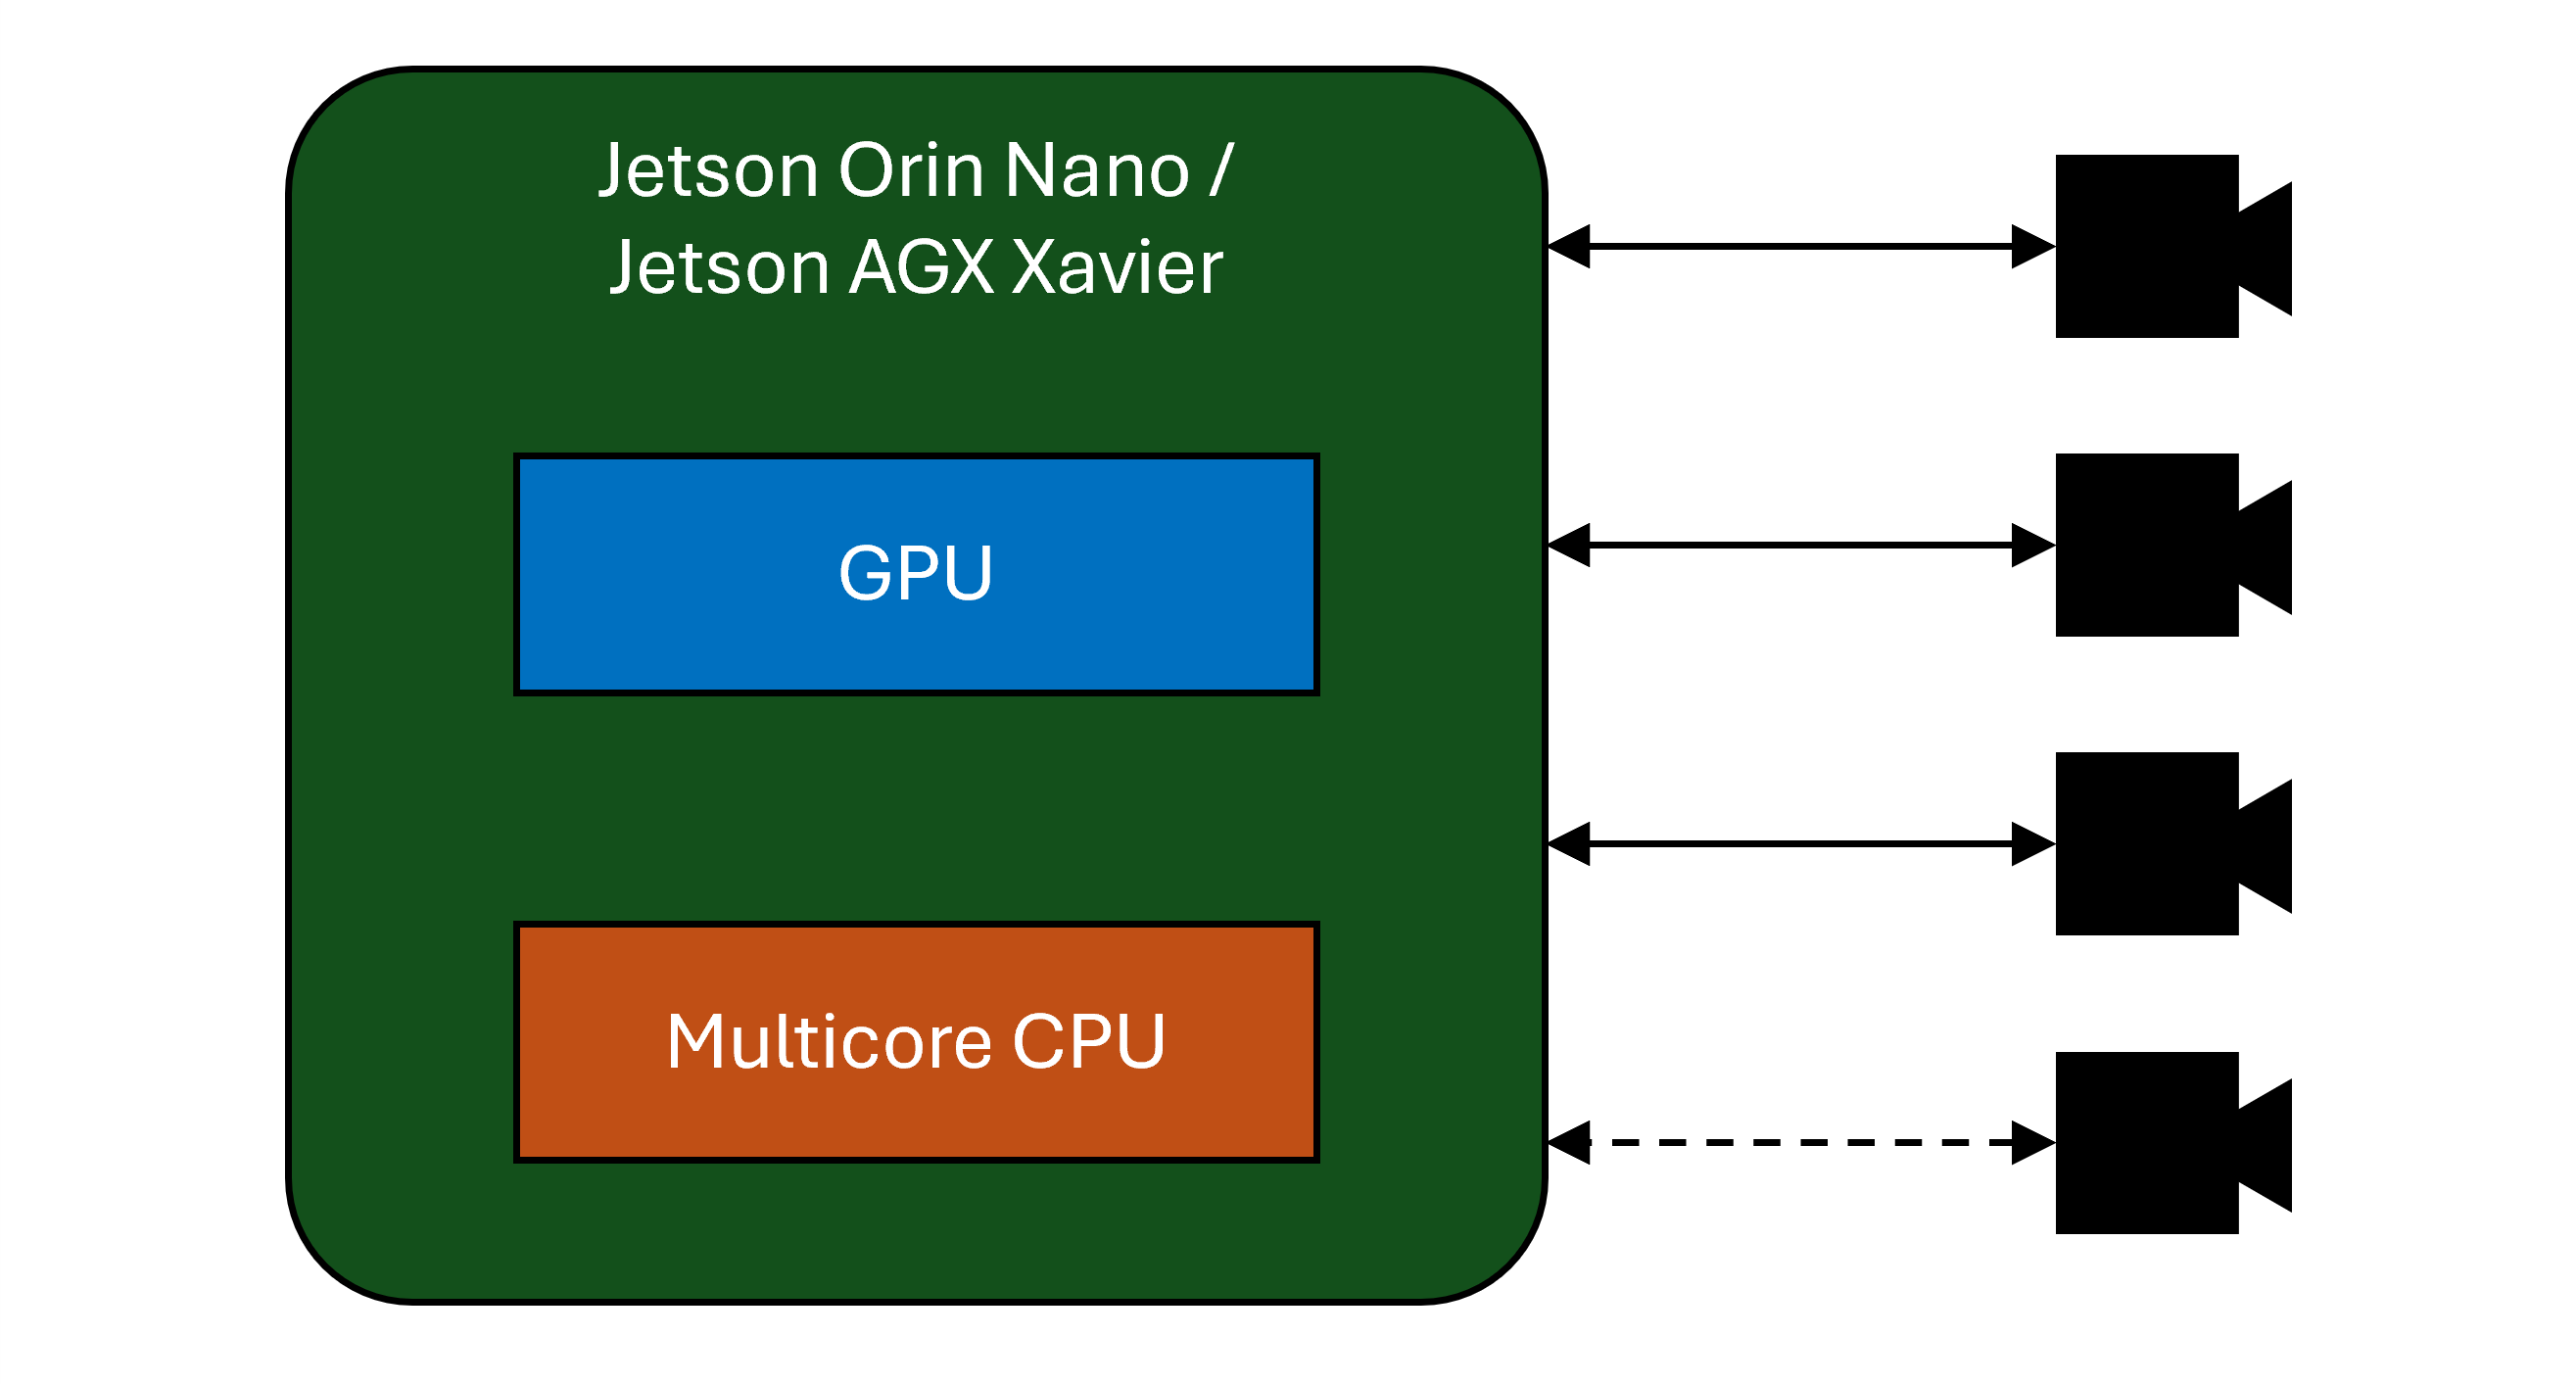
\includegraphics[width=0.9\textwidth]{images/HW-schematics.png}}
	\caption{\centering Schematic of the hardware setup}
	\label{fig:hw-setup}
\end{figure}
